\documentclass[francais]{beamer}
\usepackage[francais]{babel}
\usepackage[utf8]{inputenc}
\usepackage[T1]{fontenc}
\usepackage{lmodern}
\usepackage{amsmath, amssymb, amsfonts}




%CHOIX DU THEME et/ou DE SA COULEUR
% => essayer différents thèmes (en décommantant une des trois lignes suivantes)
%\usetheme{PaloAlto}
\usetheme{Madrid}

% => il est possible, pour un thème donné, de modifier seulement la couleur
\usecolortheme{default}
%\usecolortheme{whale}

%\useoutertheme[left]{sidebar}


%Pour le TITLEPAGE


\title[Nicolas Baillot d'Etivaux]{Constraining the equation of state for dense matter through thermal emission of neutron stars}


%Debut de la presentation :

\begin{document}


%Présentation:
\setbeamertemplate{blocks}[rounded]%
[shadow=false]




\begin{frame}{Full resolution:}
n:
\begin{center}
 % 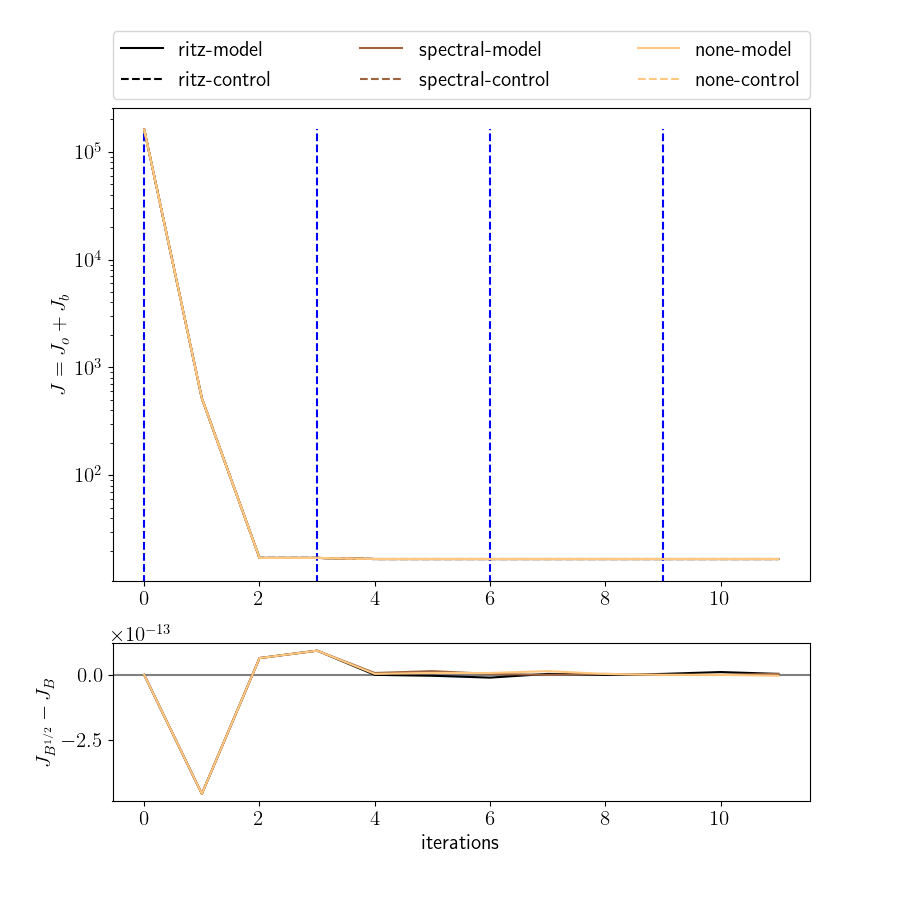
\includegraphics[scale=0.3]{./images/im1.png}
\end{center}
\end{frame}



%BACKUP SLIDES:

\usebackgroundtemplate{}




\end{document}
